%!TEX root = 00_main.tex

\section{Experiments}

%\commentA{the distribution figures would be nice here, e.g. to make the point that we can synthesise arbitrary distributions and to beef up the gaze estimation experiments}

% \begin{figure}
%     \centering
%     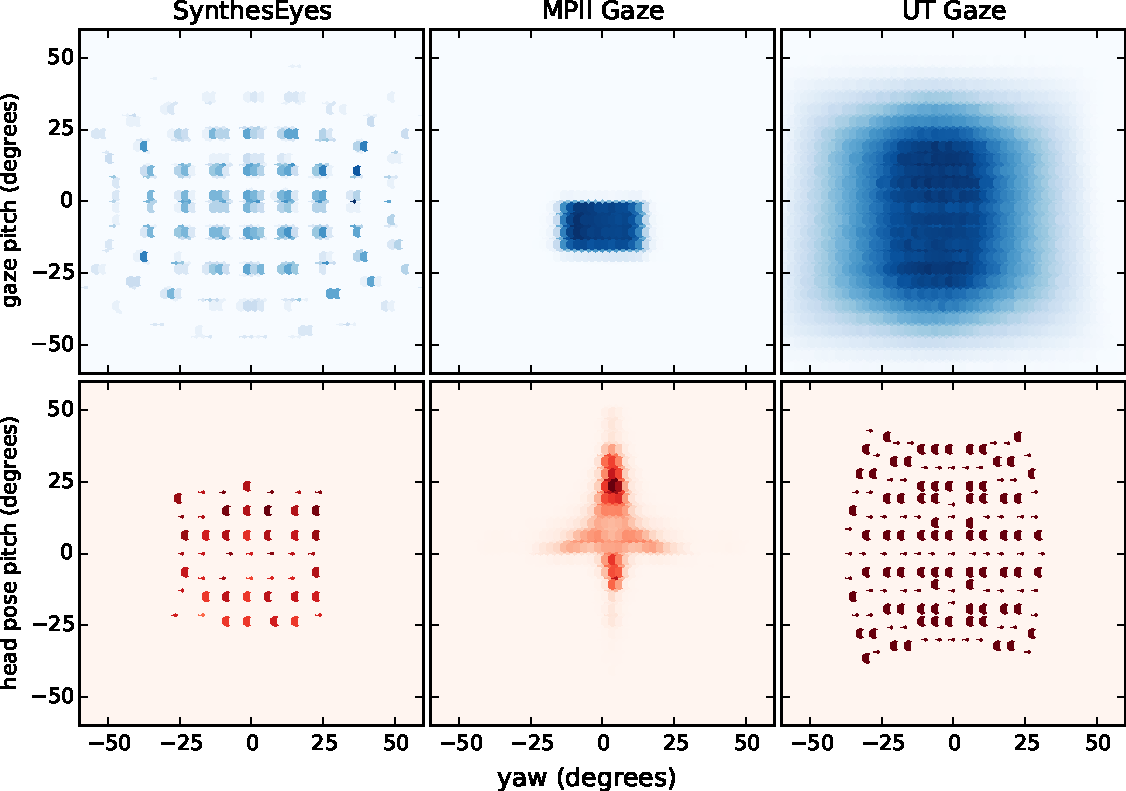
\includegraphics[width=\textwidth]{head_gaze_distribution_v2.pdf}
%     \caption{The head pose (first row) and gaze direction (second row) distribution of different datasets.}
%     \label{fig:head_gaze_distribution}
% \end{figure}

%\commentA{just a reminder to potentially remove the top row in Figure 8 (head pose distributions)}

% \begin{figure}
    \centering
    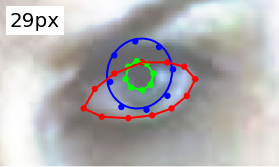
\includegraphics[width=0.244\columnwidth]{figs/wild_ldmks_examples/idx_550.png}\hfill
    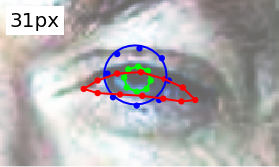
\includegraphics[width=0.244\columnwidth]{figs/wild_ldmks_examples/idx_560.png}\hfill
    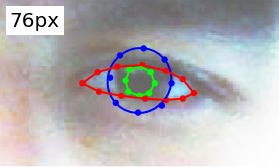
\includegraphics[width=0.244\columnwidth]{figs/wild_ldmks_examples/idx_799.png}\hfill
    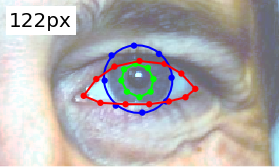
\includegraphics[width=0.244\columnwidth]{figs/wild_ldmks_examples/idx_721.png}
    \par \vspace{0.1em}
    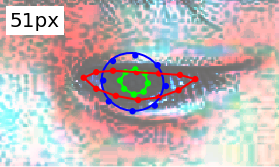
\includegraphics[width=0.244\columnwidth]{figs/wild_ldmks_examples/idx_1013.png}\hfill
    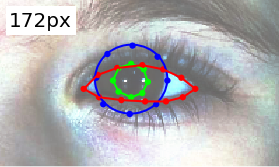
\includegraphics[width=0.244\columnwidth]{figs/wild_ldmks_examples/idx_1002.png}\hfill
    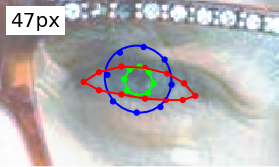
\includegraphics[width=0.244\columnwidth]{figs/wild_ldmks_examples/idx_765.png}\hfill
    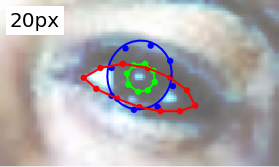
\includegraphics[width=0.244\columnwidth]{figs/wild_ldmks_examples/idx_508.png}
    \par \vspace{0.1em}
    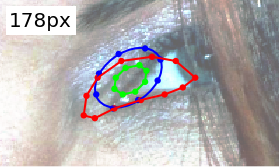
\includegraphics[width=0.244\columnwidth]{figs/wild_ldmks_examples/idx_934.png}\hfill
    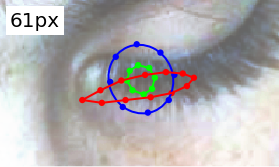
\includegraphics[width=0.244\columnwidth]{figs/wild_ldmks_examples/idx_875.png}\hfill
    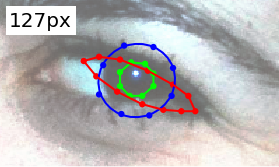
\includegraphics[width=0.244\columnwidth]{figs/wild_ldmks_examples/idx_913.png}\hfill
    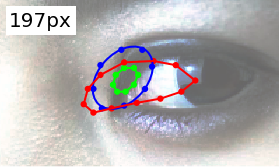
\includegraphics[width=0.244\columnwidth]{figs/wild_ldmks_examples/idx_953.png}
    %
    \caption{The top two rows illustrate successful eye-shape registration on 300-W. The bottom row illustrates failure cases, including un-modelled occlusions and eyelid poses.}
    \label{fig:example_fits_wild}
\end{figure}

% \commentA{briefly say something about significance/importance of both problems, more in corresponding subsections}

% \commentY{Maybe this should be presented earlier (in the related works section? we are currently missing references to other appearance-based gaze estimation methods), definition of the two tasks and why and how synthetic data is expected to be helpful. Especially eye-shape registration is not well defined during the previous section}
We evaluated the usefulness of our synthetic data generation method on two sample problems, eye-shape registration and appearance-based gaze estimation.

Eye-shape registration attempts to detect anatomical landmarks of the eye -- eyelids, iris and the pupil. 
Such approaches either attempt to model the shape of the eye directly by relying on low-level image features, e.g. edges \cite{wood2014eyetab, swirski2012robust} or by using statistically learnt deformable models \cite{alabort2014statistically}. 
Compared to \citet{alabort2014statistically}, our dataset has been automatically labelled. This guarantees consistent labels across viewpoints and people, avoiding human error.

Appearance-based gaze estimation systems learn a mapping directly from eye image pixels to gaze direction.
While most previous approaches focused on {\em person-dependent} training scenarios which require training data from the target user, recently more attention has been paid to {\em person-independent} training \cite{zhang15_cvpr,sugano2014learning,funes2013person,schneider2014manifold}. 
% This is in contrast to geometry-based approaches that rely on tracking features of 
%This is a challenging task considering the changes in appearance, 
%thus requiring large amounts of training data to perform well.
The training dataset is required to cover the potential changes in appearance with different eye shapes, arbitrary head poses, gaze directions, and illumination conditions.
%
%Since our method allows the synthesis of eye images with arbitrary head poses, gaze directions, and illumination conditions, we can generate a suitable training dataset rapidly, and even tailor it to the target domain.
Compared to \citet{sugano2014learning}, our method can provide a wider range of illumination conditions which can be beneficial to handle the unknown illumination condition in the target domain.

%\subsection{Eye-Shape Registration In the Wild}

\subsection{Eye-Shape Registration}

As our method can reliably generate consistent landmark location training data, we used it for training a Constrained Local Neural Field (CLNF) \cite{baltrusaitis2013constrained} deformable model. We conducted experiments to evlauate the generalizability of our approach on two different use cases: eyelid registration in-the-wild, and iris tracking from webcams.

\paragraph{Eyelid Registration In the Wild}

% \commentA{maybe this should also read eye-shape registration in both section heading and text to be consistent with the next subsection}

\begin{figure}
    \centering
    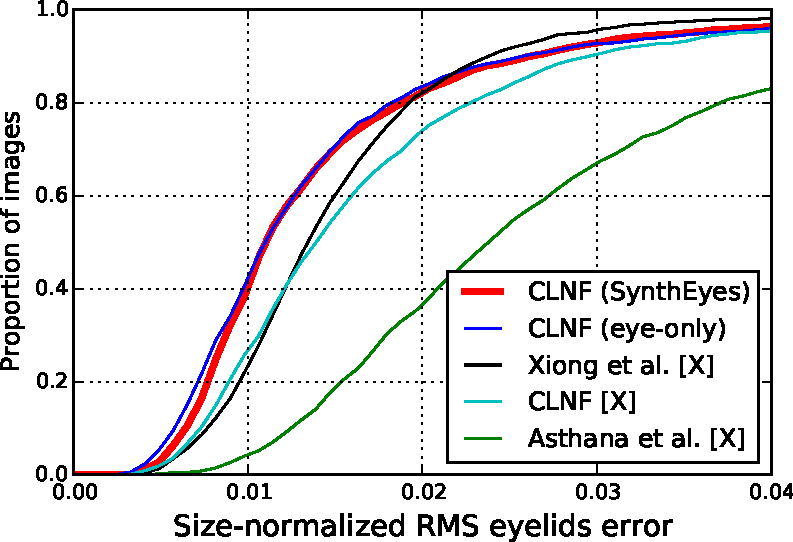
\includegraphics[width=\columnwidth]{figs/CLNF_300W_experiment.pdf}
    \caption{We outperform the state-of-the-art for eyelid-registration in the wild. The right plot shows how performance degrades for training data without important degrees of variation: realistic lighting and eyelid movement.}
    \label{fig:clnf_results_wild}
\end{figure}

% \begin{figure}
    \centering
    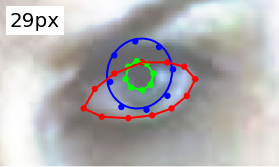
\includegraphics[width=0.244\columnwidth]{figs/wild_ldmks_examples/idx_550.png}\hfill
    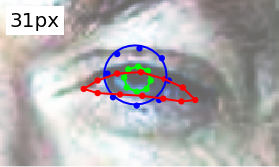
\includegraphics[width=0.244\columnwidth]{figs/wild_ldmks_examples/idx_560.png}\hfill
    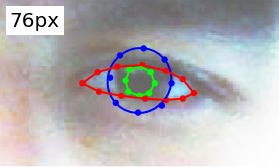
\includegraphics[width=0.244\columnwidth]{figs/wild_ldmks_examples/idx_799.png}\hfill
    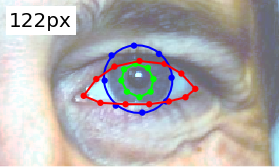
\includegraphics[width=0.244\columnwidth]{figs/wild_ldmks_examples/idx_721.png}
    \par \vspace{0.1em}
    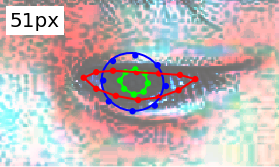
\includegraphics[width=0.244\columnwidth]{figs/wild_ldmks_examples/idx_1013.png}\hfill
    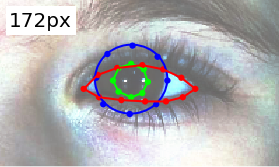
\includegraphics[width=0.244\columnwidth]{figs/wild_ldmks_examples/idx_1002.png}\hfill
    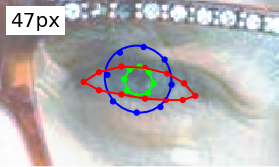
\includegraphics[width=0.244\columnwidth]{figs/wild_ldmks_examples/idx_765.png}\hfill
    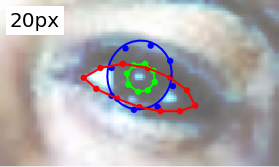
\includegraphics[width=0.244\columnwidth]{figs/wild_ldmks_examples/idx_508.png}
    \par \vspace{0.1em}
    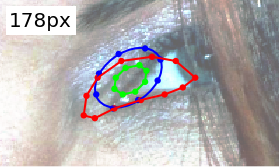
\includegraphics[width=0.244\columnwidth]{figs/wild_ldmks_examples/idx_934.png}\hfill
    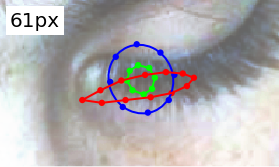
\includegraphics[width=0.244\columnwidth]{figs/wild_ldmks_examples/idx_875.png}\hfill
    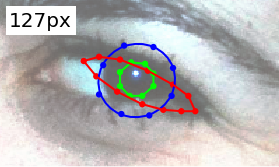
\includegraphics[width=0.244\columnwidth]{figs/wild_ldmks_examples/idx_913.png}\hfill
    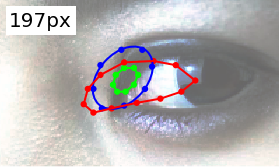
\includegraphics[width=0.244\columnwidth]{figs/wild_ldmks_examples/idx_953.png}
    %
    \caption{The top two rows illustrate successful eye-shape registration on 300-W. The bottom row illustrates failure cases, including un-modelled occlusions and eyelid poses.}
    \label{fig:example_fits_wild}
\end{figure}

% Erroll to Tadas: need to make sure these facts are straight...
We performed an experiment to see how our system generalises on unseen and unconstrained images. We used the validation datasets from the 300 Faces In-the-Wild (300-W) challenge \cite{sagonas2013300} which contain labels for eyelid boundaries. We tested all of the approaches on the 830 (out of 1026) test images. We discarded images that did not contain visible eyes (occluded by hair or sunglasses) or where face detection failed for other comparison systems used in our experiment.
% This lead to 1660 eye images for evaluation.

We trained CLNF patch experts using the generic \dataset dataset and used the 3D landmark locations to construct a Point Distribution Model (PDM) using Principal Component Analysis. 
As our rendered images did not contain closed eyes we generated extra closed eye landmark labels by moving the upper eyelid down to lower one or meeting both eyelids halfway.
We initialised our approach by using the face-CLNF \cite{baltrusaitis2013constrained} facial landmark detector.
To compare using synthetic or real training images, we trained an eyelid CLNF model on 300-W images, but used the same PDM used for synthetic data (CLNF 300-W).
We also compared our approach with the following state-of-the-art facial landmark detectors trained on in-the-wild data: CLNF \cite{baltrusaitis2013constrained}, Supervised Descent Method (SDM) \cite{Xiong2013sdm}, Discriminative Response Map Fitting (DRMF) \cite{Asthana2013drmf}, and tree based face and landmark detector \cite{Zhu2012tree}. 

The results of our experiments can be seen in \autoref{fig:clnf_results_wild}, and example model fits are shown in \autoref{fig:fits_300W}.
Errors were recorded as the RMS point-to-boundary distance from tracked eyelid landmarks to ground truth eyelid boundary, and were normalized by inter-ocular distance. 
%
First, our system CLNF Synth ($\mathrm{Mdn}=0.0110$) trained on only ten participants in four lighting conditions results in very similar performance to a system trained on unconstrained in-the-wild images, CLNF 300-W ($\mathrm{Mdn}=0.0110$).
%
Second, the results show the eye-specific CLNF outperformed all other systems in eye-lid localization: SDM ($\mathrm{Mdn}=0.0134$), face-CLNF ($\mathrm{Mdn}=0.0139$), DRMF ($\mathrm{Mdn}=0.0238$), and Tree based ($\mathrm{Mdn}=0.0217$). 
% and that our system can be used to achieve state-of-the-art performance for eye shape registration. 
%Furthermore, our approach managed to generalise without explicit modelling of eye-glasses or other partial occlusions.
The frist result suggests the importance of high-quality consistent labels. In addition, we perform well despite the fact our models do not exhibit emotion-related shape deformation, such as brow-furrowing, squinting, and eye-widening.

Our approach also allow us to examine what steps of the synthesis are important for generating good training data. We trained two further eye-specific CLNFs on different versions of \dataset, one without eyelid motion and one with only one fixed lighting condition. As can be seen in \autoref{fig:clnf_results_wild}, not using shape variation ($\mathrm{Mdn}=0.0129$) and using basic lighting ($\mathrm{Mdn}=0.0120$) lead to worse performance due to missing degrees of variability in training sets.

%\subsection{Eye-Shape Registration for Webcams}
\paragraph{Eye-Shape Registration for Webcams}

% \commentA{``for laptops'' sounds very specific. Does this generalise, do we need this strong constraint?}

%!TEX root = ../00_main.tex

%
\begin{figure*}[ht]
    \captionsetup[subfigure]{labelformat=empty} % stop subcaption writing "(a)""
    \captionsetup{subrefformat=parens} % add parentheses to \subref
    \centering
    \begin{subfigure}[t]{\columnwidth}
        \inlinelabel{a}{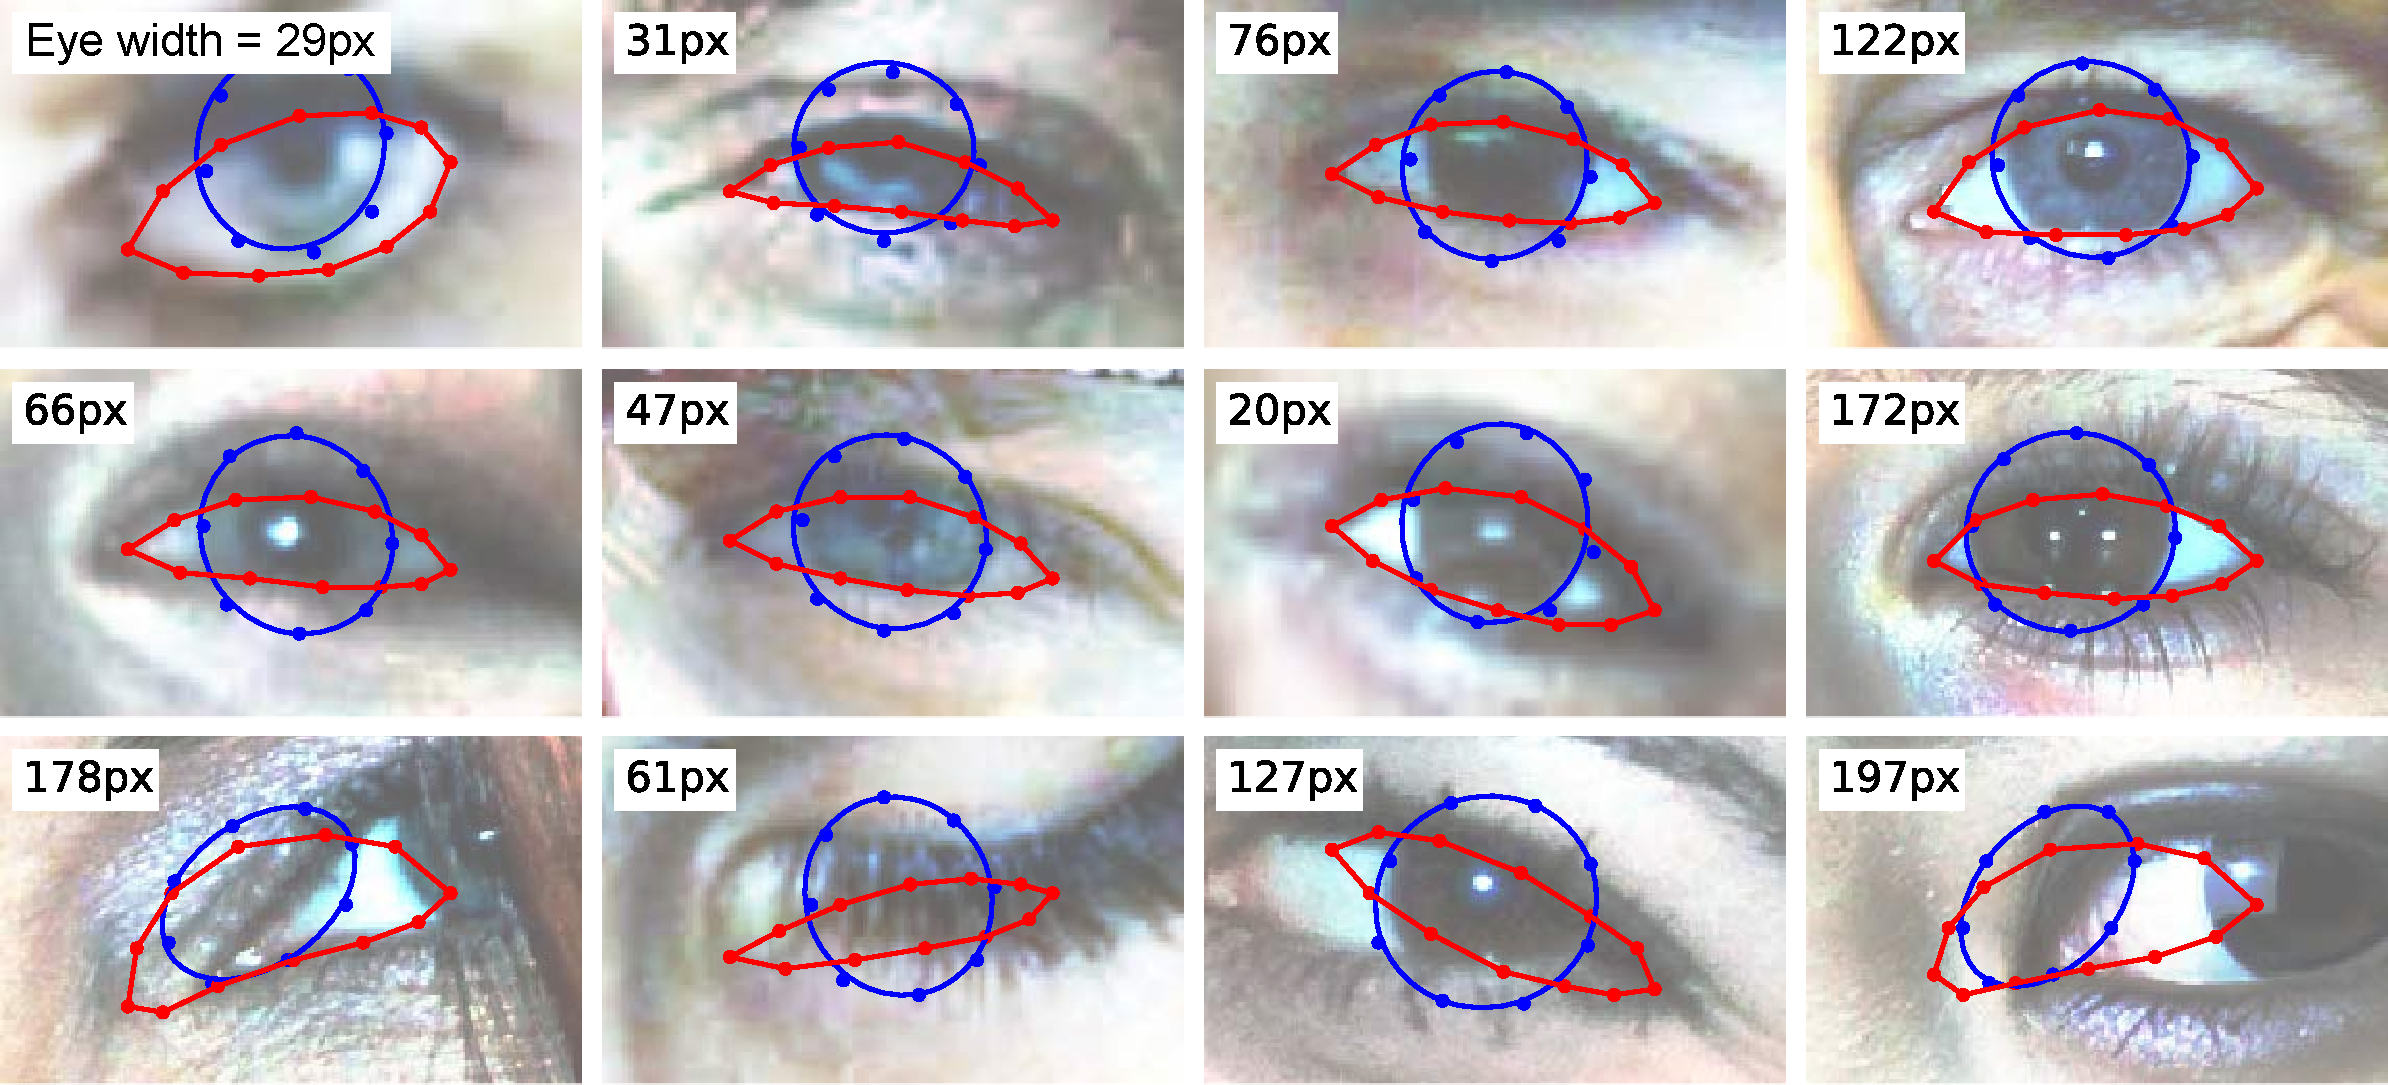
\includegraphics[width=\textwidth]{fits_300W}}
        \caption{}\label{fig:fits_300W}
    \end{subfigure}
    \hfill
    \begin{subfigure}[t]{\columnwidth}
        \inlinelabel{b}{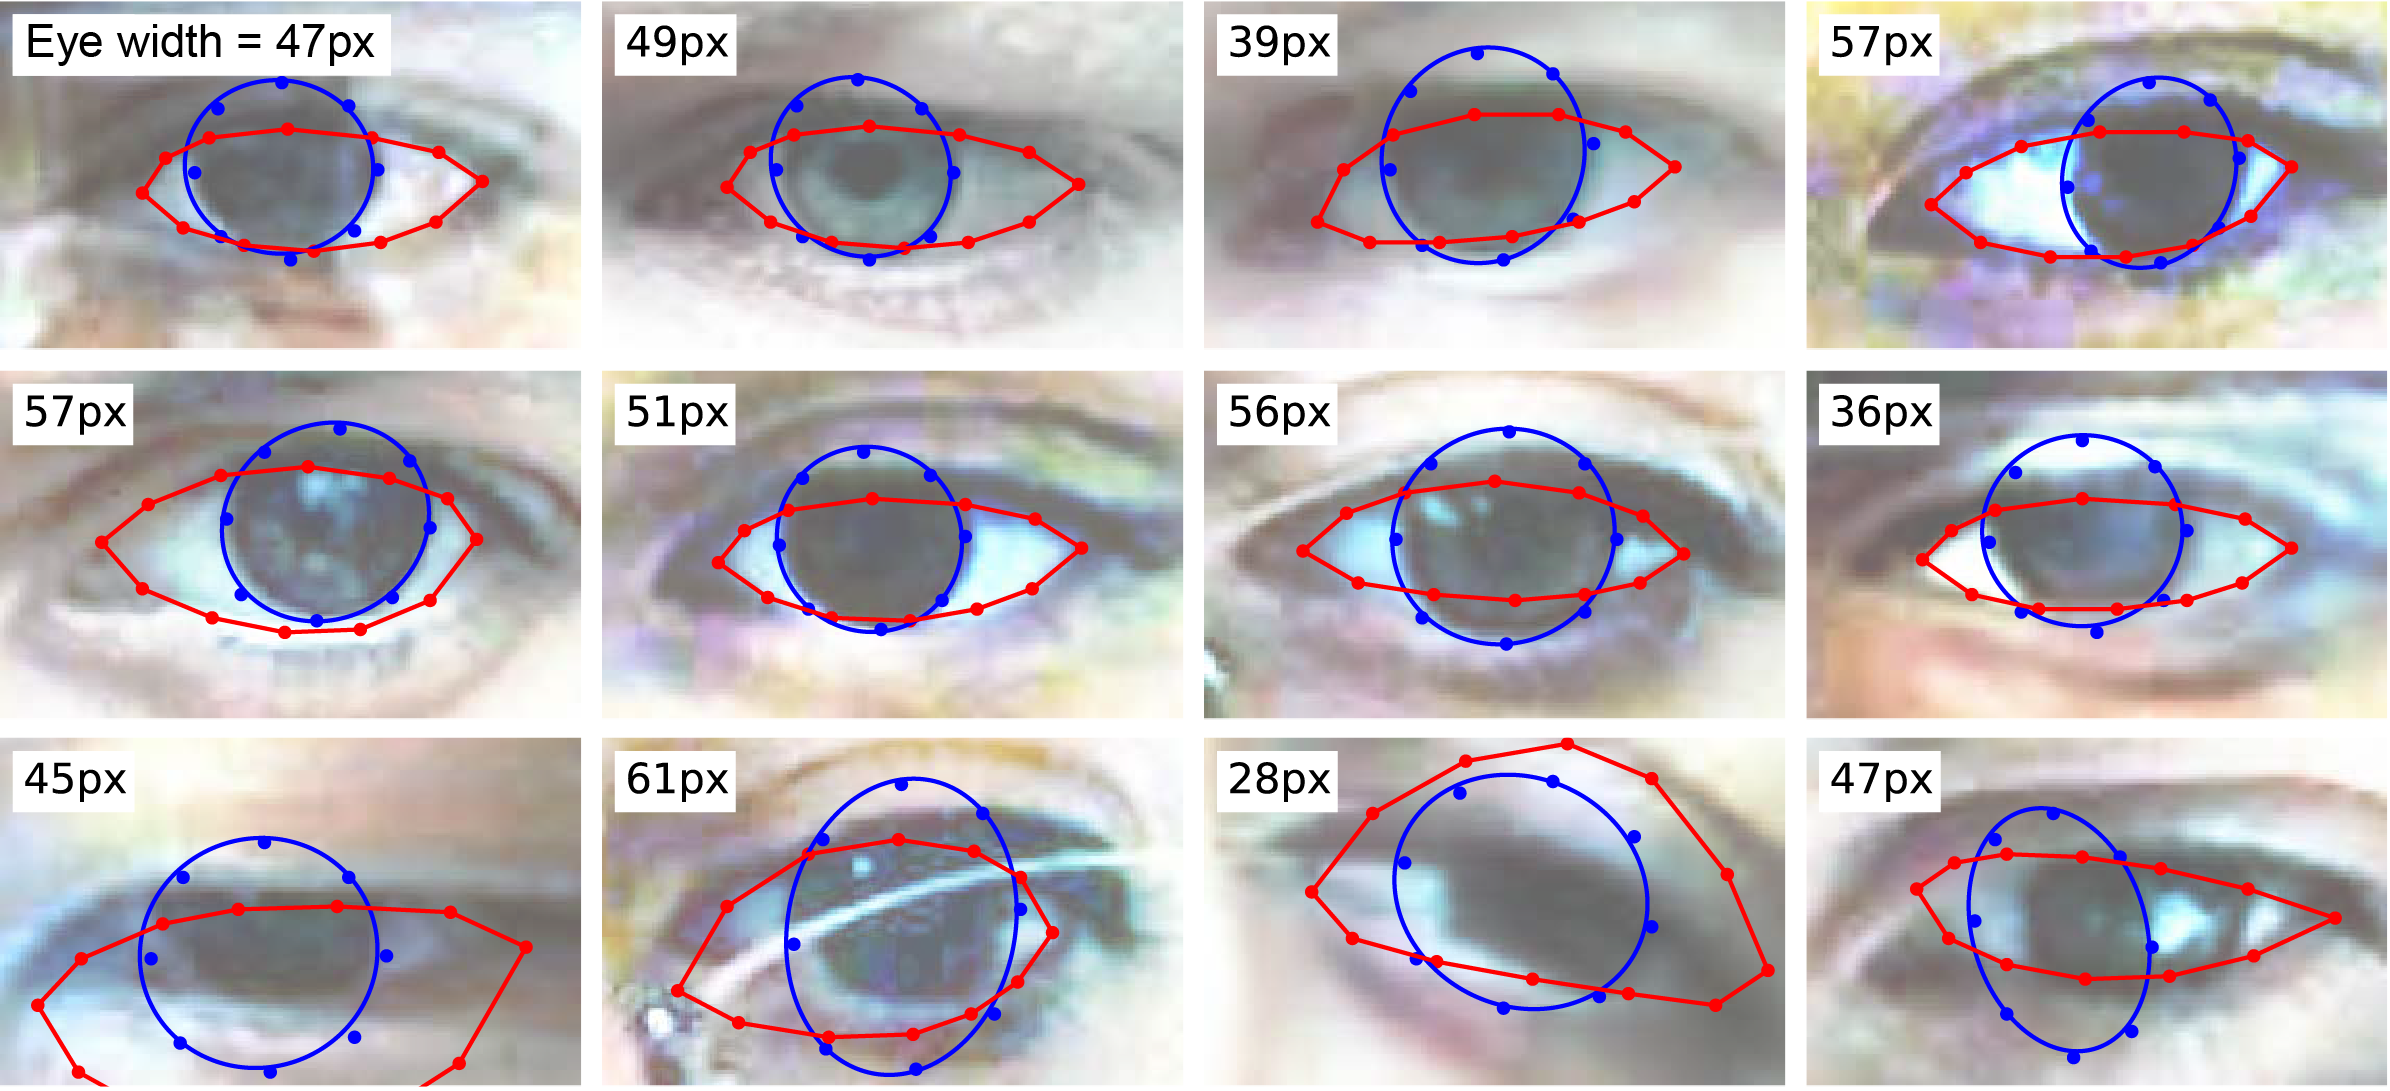
\includegraphics[width=\textwidth]{fits_MPII}}
        \caption{}\label{fig:fits_MPII}
    \end{subfigure}
    \par\vspace{-28pt}
    \caption{Example fits of our eye-CLNF trained on \dataset on in-the-wild images \subref{fig:fits_300W} and webcam images \subref{fig:fits_MPII}. The top two rows illustrate successful eye-shape registration, while the bottom rows illustrate failure cases, including unmodelled occulsions (hair), unmodelled poses (fully closed eye), glasses, and incorrect model initializaion.}
    \label{fig:example_fits}
\end{figure*}

\begin{figure}
    \centering
    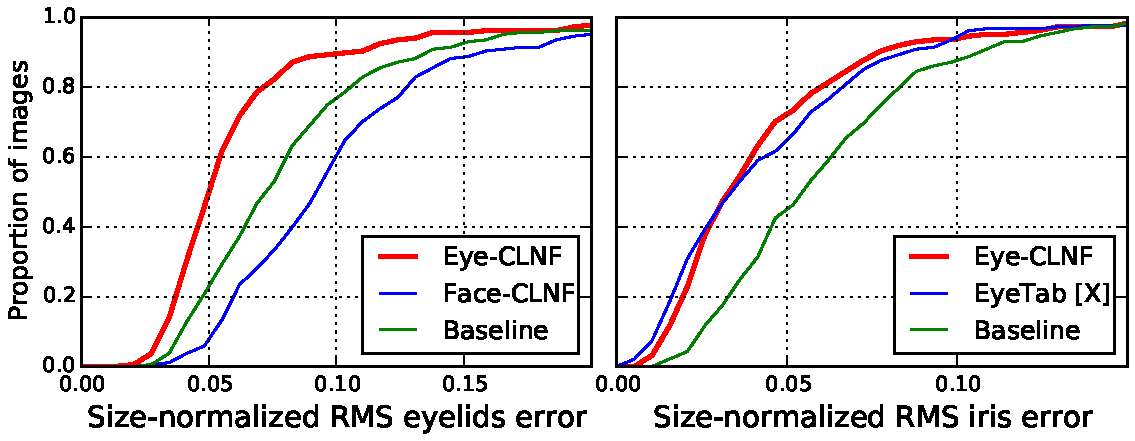
\includegraphics[width=\columnwidth]{CLNF_MPII_experiment}
    \caption{We perform comparably with state-of-the-art for iris-registration on in-the-wild webcam images.}
    \label{fig:clnf_results_MPII}
\end{figure}

While the 300-W images represent challenging conditions for eyelid registration they do not feature iris labels and are not representative of conditions encountered during everyday human-computer interaction.
We therefore annotated sub-pixel eyelid and iris boundaries for a subset of MPIIGaze \cite{zhang15_cvpr} (188 images), a recent large-scale dataset of face images and corresponding on-screen gaze locations collected during everyday laptop use over several months \cite{zhang15_cvpr}.
Pupil accuracy was not evaluated as it was impossible to discern in in most images.

We compared our eye-specific CLNF (CLNF Synth) with EyeTab \cite{wood2014eyetab}, a state-of-the-art shape-based approach for webcam gaze estimation that robustly fits ellipses to the iris boundary using image-aware RANSAC \cite{swirski2012robust}. Note we did not compare with other systems from the previous experiment as they do not detect irises.
We used a modified version of the author's implementation with improved eyelid localization using CLNF \cite{baltrusaitis2013constrained}.
As a baseline, we used the mean position of all 28 eye-landmarks following model initialization.
Eyelid errors were calculated as RMS distances from predicted landmarks to the eyelid boudnary.
Iris errors were calculated by least-squares fitting an ellipse to the tracked iris landmarks, and measuring distances only to visible parts of the iris.
%discretizing it, removing points outside ground truth and tracked eyelid boundaries, and then measuring RMS distances to the ground truth iris.
% This avoided calculating errors for parts of the iris which were occluded by the eyelid.
Errors were normalized by the eye-width, and are reported using average eye-width ($44.4\textrm{px}$) as reference.

As shown in \autoref{fig:clnf_results_MPII}, our approach ($\textrm{Mdn}\!=\!1.48\textrm{px}$) demonstrates comparable iris-fitting accuracy with EyeTab ($\textrm{Mdn}\!=\!1.44\textrm{px}$).
%a state-of-the-art algorithm for fitting ellipses to irises in low-quality images.
However, CLNF Synth is more robust, with EyeTab failing to terminate in $2\%$ of test cases.
As also shown by the 300-W experiment, the eye-specific CLNF Synth localizes eyelids better than the face-CLNF.
See \autoref{fig:fits_MPII} for example model fits.
%As shown by \todo{prev exp.}, our eye-CLM ($2.79\!\pm\!2.20\textrm{px}$) also localizes eyelids better than previous state-of-the-art facial landmark trackers ($4.27\!\pm\!1.84\textrm{px}$).

% show that we only need data from few(er) people and show competitive performance
% Maybe) Plot landmark accuracy on LFW against number of training participants. Show that even with just a few participants (e.g. 4) we get good results for eyelid positions compared to state-of-the-art face trackers.

% eye corner detection
% eye bounding box detection
% eye position detection?
% ^ I think all of these come with what the deformable model gives us

\subsection{Appearance-Based Gaze Estimation}

% evaluate eye/gaze/eyelid shapes (fully synthetic) separately from full face appearance (which is a mixture of real and synthetic data)

% person-adaptation, use pre-trained model from synthesised data, then personalise with small amount of user-specific data
% ^ let's leave this as future work! Can put it in the discussion 

% show that we can synthesise specific datasets for specific settings (specific head and gaze ranges, illumination conditions), show that we can competitive performance

\begin{figure}
    \centering
    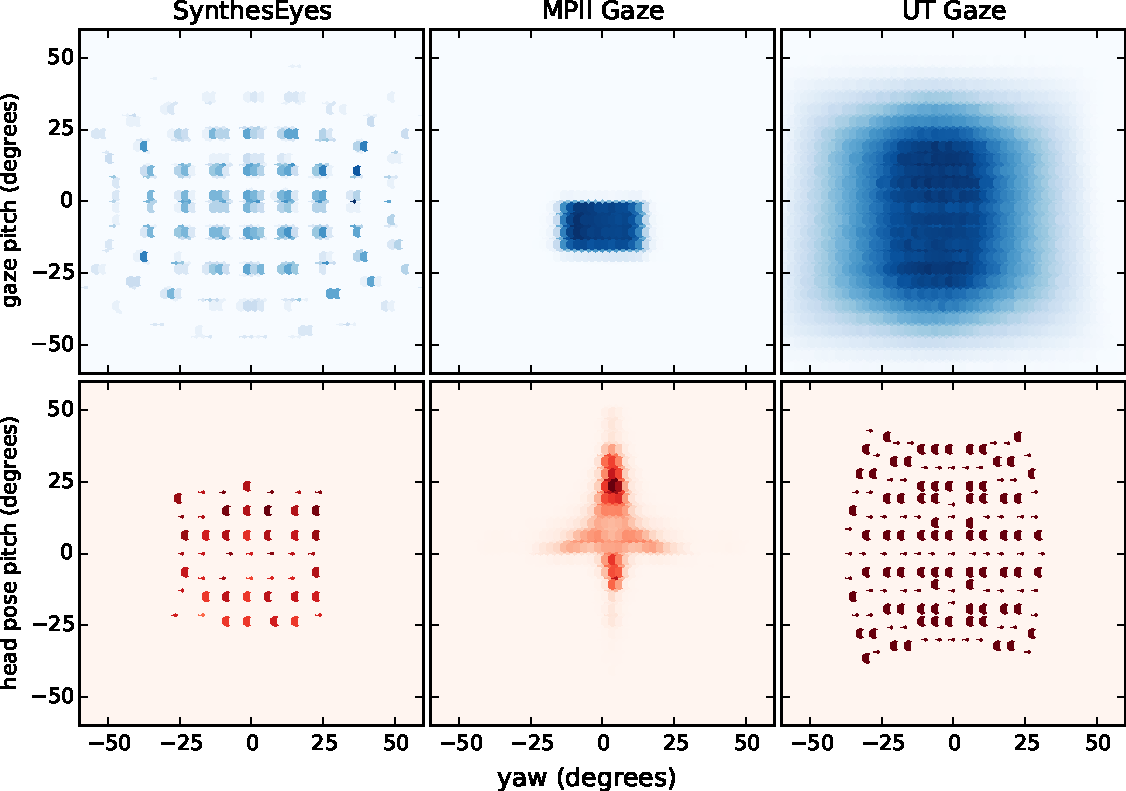
\includegraphics[width=0.9\columnwidth]{head_gaze_distribution_v2.pdf}
    \caption{The gaze direction (first row) and head pose (second row) distributions of different datasets: \dataset, MPIIGaze~\cite{zhang15_cvpr}, and UT Multiview \cite{sugano2014learning}.}
    \label{fig:head_gaze_distribution}
\end{figure}

\begin{figure}
    \centering
    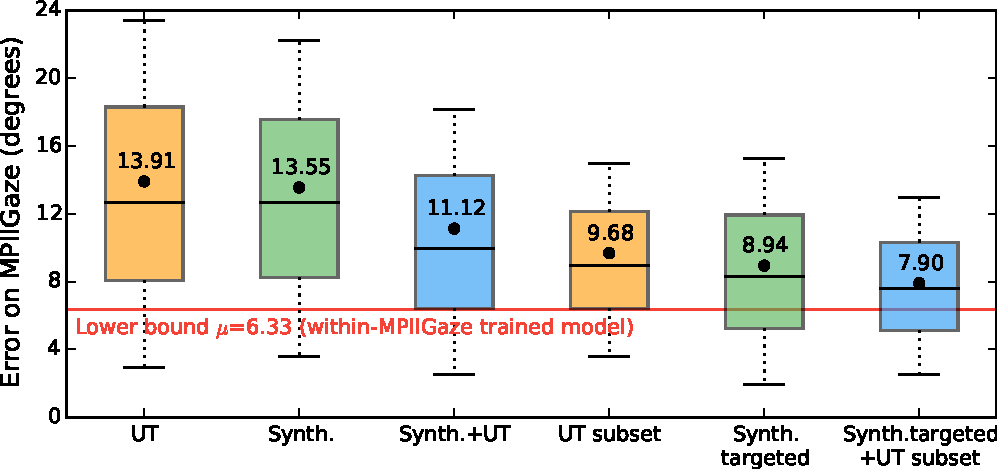
\includegraphics[width=\columnwidth]{gazeResult_v3.pdf}
    \caption{Gaze estimation performance on MPIIGaze using different datasets for training. Black dots are mean errors, and red line represents a practical lower-bound (within-dataset cross-validation score). Note how combining synthetic datasets for training leads to improved performance (blue plots).}
    \label{fig:gazeResult}
\end{figure}

%\commentY{Edited this paragraph}
To evaluate the suitability of our synthesis method for appearance-based gaze estimation we performed a cross-dataset experiment as described by \citet{zhang15_cvpr}.
%where they trained and tested the model on different datasets. 
We synthesized training images using the same camera settings as in the UT dataset~\cite{sugano2014learning}.
% We did not do this.
% and used the same normalization scheme for the test data.
The head pose and gaze distributions for the three datasets are shown in~\autoref{fig:head_gaze_distribution}.
%The training data was fully compatible with UT dataset, and
We then trained the same convolutional neural network (CNN) model as described by~\citet{zhang15_cvpr} on both synthetic datasets and evaluated their performance on MPIIGaze.

%Following the same setting, we train the same Convolutional Neural Network (CNN) model on the generic~\dataset dataset, and test it on MPIIGaze evaluation subset proposed by~\cite{zhang15_cvpr}. 
As shown
%with the two bars at the far left o
in~\autoref{fig:gazeResult}, the CNN model trained on our generic~\dataset dataset achieved similar performance ($\mu\!=\!13.91^{\circ}$) as the model trained on the UT dataset \mbox{($\mu\!=\!13.55^{\circ}$)}.
%\commentE{I will prepare numbers here}
This confirms that our approach can synthesise data that leads to comparable results with previous synthesis procedures \cite{sugano2014learning}.
% We're finding it hard to argue why SynthEyes is better than UT, but maybe thats OK
Note from \autoref{fig:gazeResult} that there is still a performance gap between the within-dataset training (blue line) and training with an external dataset.
% The blue line in~\autoref{fig:gazeResult} shows the leave-one-person-out cross validation score within the MPIIGaze dataset and thus represents the lower bound in this evaluation scenario.
These results suggest that both the \dataset~and UT datasets do not capture all variations present in the test set. For example we do not model eye-glasses and the distortions caused by them; camera-related effects such over and under-exposure; and we do not capture all possible eye-shape variations.
% still have error sources that cause this performance gap.
% \commentA{are these values comparable in terms of training setting etc to fig 7 in the CVPR paper? I feel we need to link these results to that work here, either for the estimation accuracy or the lower bound.}

%\paragraph{Head Pose and Gaze Ranges}
%To better model the variations encountered for everyday laptop-use images, we 

% One of the important factors related to the above gap is the head pose and gaze ranges.
While it is important to cover a wide range of head poses to handle arbitrary camera settings, this can make the training task more difficult.
If the target setting is known in advance, e.g. laptop gaze interaction, it is  possible to target the synthesis of training data to the expected head pose and gaze ranges.
%The head pose and gaze direction range are also quite important priors for appearance-based gaze estimation. 
%Since the samples from the small range of head poses can be trained together, while extreme head poses wouldn't share eye appearance. Also the gaze direction space is arbitrary and difficult to be densely covered by collected dataset.
To analyse the effect of different head pose ranges we rendered an additional targeted dataset (\dataset targetted) for a typical laptop setting ($10^{\circ}$ pose variation, $20^{\circ}$ gaze variation).
%Notice that the head pose and gaze direction range can be estimated based on the task, so the required information is not sophisticated. 
%This shows how we can target specific scenarios like laptop-based gaze estimation, and render a suitable dataset within a day rather than taking 3 months of data collection with 15 participants. 
For comparison, we also re-sampled the entire UT dataset to create a subset (UT subset) that has the same gaze and head pose distribution as MPIIGaze.
% as described by~\citet{zhang15_cvpr}.
%A second important difference between two datasets is the number of subjects in the dataset.
%Since there are just have 10 subjects in our~\dataset,
To make the comparison fairer, we divided the UT subset into five groups with 10 subjects each,
%(15,000 samples per group, as with our~\dataset).
and then averaged the performance of the five groups for the final result. 
As shown in the third and forth bars of~\autoref{fig:gazeResult}, having similar head pose and gaze direction ranges as the target domain improves performance compared to the generic datasets.
%$\textrm{Mdn}\!=\!8.95^{\circ}$ and $\textrm{Mdn}\!=\!8.29^{\circ}$ for UT and \dataset respectively.
Trained on our \dataset dataset the CNN achieves a statistically significant performance improvement over the UT dataset of 0.74$^{\circ}$ (Wilcoxon signed-rank test  $p\!<\!0.0001$).
% $\textrm{Mdn}\!=\!8.95^{\circ}$ and $\textrm{Mdn}\!=\!8.29^{\circ}$ for UT and \dataset respectively.

As shown in \autoref{fig:gazeResult}, it is possible to achieve better performances (untargetted $\mu\!=\!11.12^{\circ}$, targetted $\mu\!=\!7.90^{\circ}$) when we train with both datasets (pre-train with \dataset, and then fine tune with UT), perhaps because they capture different degrees of variation.
%Interestingly pre-training using UT followed by \dataset led to worse performance. This indicates further need to investigate best strategies for dataset combination.

% Erroll: not sure about the below paragraph
% Since both UT subset and~\dataset subset have the similar head pose and gaze direction range, the performance gains should come from the realistic samples generate from precise 3D eye model and also simulated variant appearance caused by light conditions.
% This result indicates, under the condition with the same number of face variations, our~\dataset subset can be a better training set compared to UT subset.

% \paragraph{Difference Between Synthesis and Realistic Data}
% The UT dataset is synthetically generated based on collected data, while our~\dataset is purely synthesis, the different affect between them for the gaze estimation training is interesting. We thus based on the the above experiments to play around their roles in such cross datasets scenario.
% We use the pre-trained model on the~\dataset and fine tune it with the UT dataset to test on MPIIGaze dataset, it is the case that we can pre-train the model with the synthetic~\dataset and fine tune the model if we have more realistic data. For caparison, we test the opposite way, i.e. pre-train the model in UT dataset and fine tune it with the~\dataset. As shown in~\autoref{tab:Synthesis_Realistic_Gaze}, our~\dataset is suitable as training data due to its generality while UT doesn't have such quality. 

\begin{figure}
    \centering
    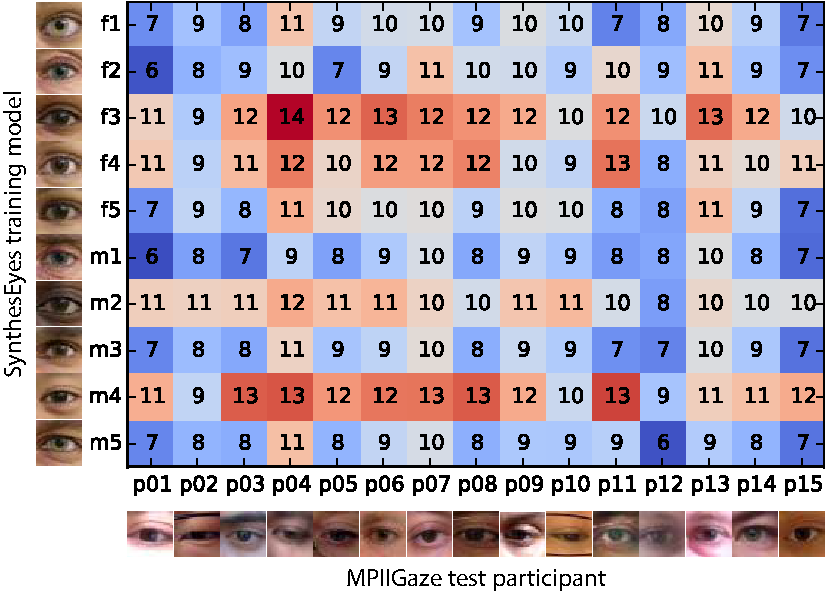
\includegraphics[width=\columnwidth]{Confusion_annotated_smallfile.pdf}
    \caption{Per-eye-model gaze estimation performance on MPIIGaze. Red represents worst scores. Note how some eye-models have proved more useful than others.
    %\commentT{Does it matter that it's left eye for some right eye for others in the small images?}
    }
    \label{fig:person_specific_training}
\end{figure}

% \begin{table}
% \begin{center}
% \begin{tabular}{ |c|p{80pt}|p{80pt}| } 
%  \hline
%  Train set & pre-train~\dataset and fine tune with UT & pre-train UT and fine tune with~\dataset \\ 
%  \hline
%  Full & X.X & X.X \\ 
%  \hline
%  Subset & 7.8 & 8.8 \\ 
%  \hline
% \end{tabular}
% \caption{The difference of pre-training on different dataset. The first row show we use the full~\dataset and full UT; The second row show the experiment done with~\dataset subset and UT subset.} 
% \label{tab:Synthesis_Realistic_Gaze}
% \end{center}
% \end{table}

\paragraph{Person-Specific Appearance}

Appearance-based gaze estimation performs best when trained and tested on the same person, as the training data includes the same eye-shape appearances that occur during testing.
However, eye-region images from \dataset and MPIIGaze can appear different due to differences in eye-shape and skin color.
To examine the effects of this we conducted a second experiment where we trained 10 separate systems (one trained on each \dataset eye model) and tested on each participant in MPIIGaze.
%, recording average error for each participant.
The results can be seen in \autoref{fig:person_specific_training}.

This plot illustrates which \dataset eye-region models were useful for training and which ones were not.
As we can see, training with certain eye models leads to poor generalization, for example \texttt{f3}, \texttt{m2}, and \texttt{m4}, perhaps due to differences in skin-tone and eye shape.
% Similarly, learning with an Asian-shaped eye-region model (m4) leads poor performance for non-Asian-shape eye-region test participants.
Also, total errors for some target participants are lower than for others, perhaps because of simpler eye-region shape that is matched to the training images.
%``easier'' eye-regions than others, e.g. ones with a plain appearance (p15).
Although intuitive, these experiments further confirm the importance of correctly covering appearance variations in the training data.
They also open up potential directions for future work, including person-specific adaptation of the renderings as well as the gaze estimator.

% Besides head pose and gaze direction ranges, it is well known that person-dependent is always the essayist scenario for gaze estimation, since the similar appearance would make the task much easier. To avoid the tedious personal calibration or long term personal data collection, one option is to use the most similar personal appearance from the training data for testing on target person. However, such training samples selection is limited inside the collected training data. Our method could generate any kind of personal appearance and do not have such limitation. As shown in~\autoref{fig:person_specific_training}, there are some subjects that suitable as training set for the MPIIGaze dataset, such as subject 1, 2, 6, 8 and 10. We use these subjects as the training set and can achieve X.X degrees on the MPIIGaze dataset.


% \begin{table}
% \begin{center}
% \begin{tabular}{ |c|c|c|c|c|c| } 
%  \hline
%  Subject ID & 1 & 2 & 3 & 4& 5 \\ 
%  \hline
%  Error & 8.5 & 9.0 & 11.65 & 10.72 & 9.3 \\ 
%  \hline
%  \hline
%  Subject ID & 6 & 7 & 8 & 9 & 10 \\ 
%  \hline
%  Error & 8.3 & 10.4 & 8.5 & 11.1 & 8.6 \\ 
%  \hline
% \end{tabular}
% \caption{The test results on MPIIGaze dataset with the training on individual subjects from~\dataset}
% \label{tab:personal_specific}
% \end{center}
% \end{table}

% \paragraph{Realism and Light Conditions}
% To test the influence of realism and light condition factors, we use the subsets of those datasets that just include frontal face clusters. We first randomly select 10 subjects from UT dataset, and take the frontal pose with their 160 gaze directions as UT frontal subset. Then we generate a~\dataset frontal subset that has the same head pose and gaze distribution with the UT frontal subset in three setting: with varying light conditions, without varying light conditions and without eyelid movement. The test set is the samples in MPIIGaze with head pose within $\pm$ 5 degrees of frontal head pose. The results are shown in~\autoref{tab:frontal_160}.

% \begin{table}
% \begin{center}
% \begin{tabular}{ |c|c| } 
%  \hline
%  Train Set & Estimation Error \\ 
%  \hline
%  SynthEye with varying light condition & 6.8 \\ 
%  \hline
%  SynthEye without varying light condition & 6.7 \\ 
%  \hline
%  SynthEye without eyelid movement & 6.8 \\
%  \hline
% \end{tabular}
% \caption{Result on realism and light conditions}
% \label{tab:frontal_160}
% \end{center}
% \end{table}

% train on synthesised images and show competitive performance on MPIIgaze with real images
% show better performance than UT dataset
%Using Xucong's CNN sytem, we train on targeted version of \dataset, test on MPII. Show results are better than training on UT and testing on MPII. This shows that the range of lighting in \dataset is important for better results.

% does photorealistic data really help/is it necessary? either reduce quality and see how it affects performance, or compare model with and without shape variations
% ^ I am not really sure how to do this well... Because we'd also have to have a measure of "how photorealistic" something is. Swapping the eyeball for a simpler model, e.g. sphere might not really have that much of an effect on "photorealism" for many eye-poses. Changing the shaders, e.g. pretending the skin is Lambertian (diffuse) might?

% \commentY{Reminder: ideally we should have a discussion on potential limitations of the current approach}

